\documentclass[final]{siamltex}

% for red MarginPars
\usepackage{color}

% for \boldsymbol
\usepackage{amsmath}
\usepackage{latexsym}
\usepackage{graphicx}
\usepackage{geometry}
\usepackage{hyperref}

% total number of floats allowed on a page
\setcounter{totalnumber}{100}

% float page fractions
\renewcommand{\topfraction}{0.9}
\renewcommand{\bottomfraction}{0.9}
\renewcommand{\textfraction}{0.2}

% MarginPar
\setlength{\marginparwidth}{0.75in}
\newcommand{\MarginPar}[1]{\marginpar{\vskip-\baselineskip\raggedright\tiny\sffamily\hrule\smallskip{\color{red}#1}\par\smallskip\hrule}}

% for non-stacked fractions
\newcommand{\sfrac}[2]{\mathchoice
  {\kern0em\raise.5ex\hbox{\the\scriptfont0 #1}\kern-.15em/
   \kern-.15em\lower.25ex\hbox{\the\scriptfont0 #2}}
  {\kern0em\raise.5ex\hbox{\the\scriptfont0 #1}\kern-.15em/
   \kern-.15em\lower.25ex\hbox{\the\scriptfont0 #2}}
  {\kern0em\raise.5ex\hbox{\the\scriptscriptfont0 #1}\kern-.2em/
   \kern-.15em\lower.25ex\hbox{\the\scriptscriptfont0 #2}}
  {#1\!/#2}}

\def\1b {{\bf 1}}
\def\Ab {{\bf A}}
\def\bb {{\bf b}}
\def\Fb {{\bf F}}
\def\gb {{\bf g}}
\def\Lb {{\bf L}}
\def\mb {{\bf m}}
\def\vb {{\bf v}}
\def\wb {{\bf w}}
\def\Wb {{\bf W}}
\def\xb {{\bf x}}
\def\zb {{\bf z}}

\def\chib   {\boldsymbol{\chi}}
\def\deltab {\boldsymbol{\delta}}
\def\Gammab {\boldsymbol{\Gamma}}
\def\phib   {\boldsymbol{\phi}}
\def\Phib   {\boldsymbol{\Phi}}
\def\Psib   {\boldsymbol{\Psi}}
\def\rhob   {\boldsymbol{\rho}}
\def\Sigmab {\boldsymbol{\Sigma}}
\def\taub   {\boldsymbol{\tau}}
\def\zetab  {\boldsymbol{\zeta}}

\def\half   {\frac{1}{2}}
\def\myhalf {\sfrac{1}{2}}

\begin{document}

%==========================================================================
% Title
%==========================================================================
\title{Low Mach Number Charged Species Notes}

\maketitle

\section{Introduction}
These are working notes for our low Mach number multicomponent charged fluid code.
The algorithm is an extension of our low Mach number multicomponent code
\cite{LowMachMulti}.  The algorithmic details are described more fully in
our previous works, in particular, the spatial discretization is described in
\cite{lowMachMixing}, and the temporal discretization for binary mixtures is
described in \cite{lowMachImplicit}.  The GMRES solver for the Stokes system
in our temporal advancement scheme is described in \cite{StokesPreconditioners}.

\section{Source Code}
There are two git repositories required to build/run the code.  BoxLib is a public
repository available on github using the command:\\ \\
{\tt git clone https://github.com/BoxLib-Codes/BoxLib.git}\\ \\
If you are not familiar with BoxLib, we recommend reading the BoxLib's User's Guide
in {\tt BoxLib/Docs}.\\

FluctHydro exists on CCSE servers and you need to contact Vince/Andy to get an account
and set up permissions on gamera.  Once you do, you can obtain the repository using:\\ \\
{\tt git clone <username>@gamera.lbl.gov:/usr/local/gitroot/FluctHydro.git}\\ \\
You will now have the following directory structures (you will actually have
more subdirectories, but below are the only directories that matter for this code):\\
%%%%%%%%%%%%%%%%%%%%%%%%%%%%%%%%%%%%%
\begin{figure}[tb]
\centering
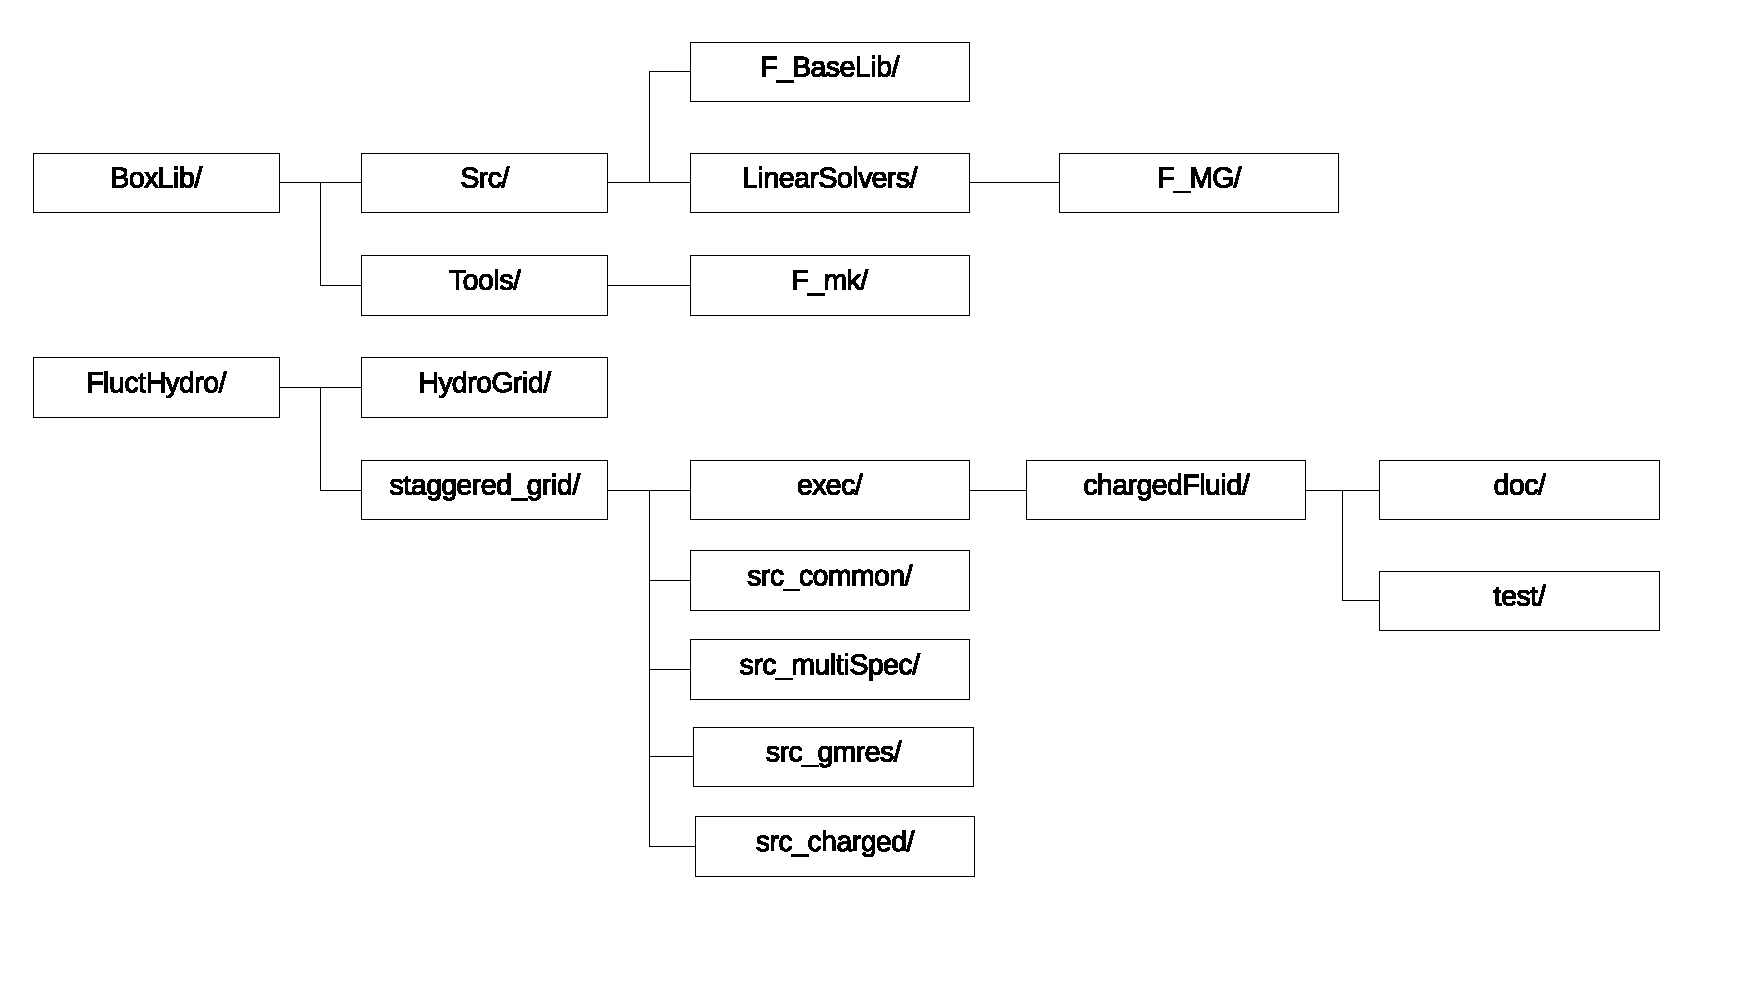
\includegraphics[width=6in]{./directory}
\caption{\label{fig:directory}Directory structure.}
\end{figure}
%%%%%%%%%%%%%%%%%%%%%%%%%%%%%%%%%%%%%
\begin{itemize}

\item {\tt BoxLib/}

\begin{itemize}

\item {\tt Src/}

\begin{itemize}

\item {\tt F\_BaseLib/}

Core libraries for parallelization of structured grid data.

\item {\tt LinearSolvers/F\_MG/}

Core libraries for linear solvers (for implicit diffusion) and diffusion stencils.

\end{itemize}
\end{itemize}

\begin{itemize}

\item {\tt Tools/F\_mk/}

Make system variables and flags.

\end{itemize}
\end{itemize}

\begin{itemize}

\item {\tt FluctHydro/}

\begin{itemize}

\item {\tt HydroGrid/}

\item {\tt staggered\_grid/}

\begin{itemize}

\item {\tt exec/charged/doc/}

Contains the document you are reading right now!

\item {\tt exec/charged/test/}

This is the compilation directory.  Contains a GNUmakefile and inputs files.

\item {\tt src\_common/}

Source code shared by all our staggered grid codes.  Contains generic namelist parameters
and routines for boundary conditions, divergence, etc.

\item {\tt src\_multiSpec/}

Source code shared by all multicomponent codes.

\item {\tt src\_gmres/}

Source code for our GMRES stokes solver.

\item {\tt src\_charged/}

Source code specific to this charged fluid problem.

\end{itemize}
\end{itemize}
\end{itemize}

\subsection{Compiling and Running}
Go to {\tt FluctHydro/staggered\_grid/exec/charged/test/} and edit the 
{\tt GNUmakefile} settings to your liking (below) and simply type {\tt `make'}.\\
\begin{verbatim}
NDEBUG    :=           # 'not debug'.  use 't' for an optimized build
MPI       := t         # use 't' to build an mpi executable
OMP       :=           # use 't' to build an OpenMP threadded executable
PROF      :=           # use 't' to turn on code profiling
COMP      := gfortran  # fortran compiler
CCOMP     := gcc       # c compiler
MKVERBOSE := t         # make verbosity

\end{verbatim}
This will generate an executable whose name provides information about the build settings,
i.e., what compiler was used, whether MPI and/or OpenMP were enabled, etc.
To run the code, simply type the executable name, followed by an inputs file.

\subsection{Input Parameters}
Refer to
\begin{itemize}
\item {\tt src\_common/probin\_common.f90}, 
\item {\tt src\_multiSpec/probin\_multiSpec.f90}, 
\item {\tt src\_gmres/probin\_gmres.f90}
\item {\tt src\_charged/probin\_charged.f90}
\end{itemize}
for namelist parameters used in the simulation and an explanation of what the parameters do.

\section{Equations}
The equations for the momentum and densities are:
\begin{eqnarray}
\frac{\partial\rho\vb}{\partial t} &=& - \nabla\cdot(\rho\vb\vb) - \nabla\pi + \nabla\cdot\taub + \rho\gb - \rho(\wb^T\zb)\nabla\Phi\\
\frac{\partial\rho_i}{\partial t} &=& -\nabla\cdot(\rho_i\vb) - \nabla\cdot\Fb_i,
\end{eqnarray}
with $\rho$ the total density, $\rho_i$ the density of component $i$, $\vb$ the fluid 
velocity, $\pi$ the perturbational pressure, $\taub$ the stress tensor, $\gb$ the
gravitational acceleration, $\wb = (w_1, w_2, \cdots)$ the vector of concentrations
(mass fractions), $\zb$ the charge per unit mass, $\Phi$ the electric potential,
and $\Fb_i$ the mass fluxes for component $i$.
Note the total charge density is $\rho(\wb^T\zb)$.

The mass fluxes include contributions from compositional gradients, barodiffusion,
thermodiffusion, electrostatic, and stochastic driving forces as described below.
The deterministic part of the mass fluxes, $\overline{\Fb}$, contains contributions from 
compositional gradients, barodiffusion, themodiffusion, and electrostatic driving forces,
\begin{equation}
\overline{\Fb} = -\rho\Wb\chib\left[\Gammab\nabla\xb + (\phib-\wb)\frac{\nabla P}{n k_B T} + \zetab\frac{\nabla T}{T} + \frac{\rho}{n k_B T}\Wb\left(\zb - (\wb^T\zb)\1b \right)\nabla\Phib\right].
\end{equation}
Note $n = \sum_i(\rho_i/w_i)$ is the number density, and 
$\rho/n = \overline{m} = (\sum_i w_i/m_i)^{-1}$ is the 
mixture-average molecular mass.
Also the total charge vector, $(\wb^T\zb){\bf 1}$, is in the null space of $\chib$,
so this term can be omitted.
The electric potential can by found by solving the Poisson equation,
\begin{equation}
-\nabla\cdot\epsilon\nabla\Phib = \rho(\wb^T\zb),
\end{equation}
with $\epsilon$ the dielectric constant.  Now the evaluation of $\Fb$
at a particular instance in time requires the solution of this Poisson equation.

The stochastic part of the mass fluxes, $\widetilde{\Fb}$, is given by,
\begin{equation}
\widetilde{\Fb} = \sqrt{2k_B}\Lb_{\half}\mathcal{Z} = \sqrt{2\bar{m}\rho}\Wb\chib_{\half}\mathcal{Z},
\end{equation}
with (see equations (28) and (29) in \cite{LowMachMulti})
\begin{equation}
\Lb_{\half} = \sqrt{\frac{\bar{m}\rho}{k_B}}\Wb\chib_{\half}
\end{equation}
In the code, we take the Cholesky factorization of $\bar{m}\rho\Wb\chib\Wb/k_B$
to obtain $\Lb_{\half}$.

The equation of state can be found by assuming no volume changing upon mixing,
and differentiating along particle paths (as in our previous low Mach mixing
papaer; will add more details):
\begin{equation}
\nabla\cdot\vb = -\nabla\cdot\left(\sum_i\frac{\Fb_i}{\bar\rho_i}\right) \equiv S\label{eq:S}.
\end{equation}

\subsection{Linearized Analysis}

\clearpage

\section{Inertial Algorithm}
Inertial algorithm description:\\ \\
{\bf Step 0: Initialization:}\\ \\
Begin with an initial guess for velocity, $\vb^{\rm init}$, and pressure, $p^0$.
Then, perform a projection to obtain an initial velocity field, $\vb^0$ that satisfies
\begin{equation}
\nabla\cdot\vb^0 = S^0 \equiv S(\Fb^0),
\end{equation}
where $\Fb_i^0$ and $\nabla\cdot\Fb_i^0$ are computed from $(\rho_i^0,T^0)$ using the 
supplied {\tt compute\_mass\_fluxdiv} subroutine.
For the projection, we solve for $\phi$ and update $\vb^{\rm init}$ as follows:
\begin{equation}
\nabla\cdot\frac{1}{\rho^0}\nabla\phi = \nabla\cdot\vb^{\rm init} - S^0,
\end{equation}
\begin{equation}
\vb^0 = \vb^{\rm init} - \frac{1}{\rho}\nabla\phi.
\end{equation}
{\bf Step 1: Calculate Predictor Diffusive and Stochastic Fluxes}\\ \\
Compute $\Fb_i^n$ and $\nabla\cdot\Fb_i^n$ from $(\rho_i^n,T^n)$ using the supplied 
{\tt compute\_mass\_fluxdiv} subroutine.  Construct $S^n$ using equation (\ref{eq:S}).
Note this step is functionally a null-op since we reuse the result from 
either {\bf Step 0} or {\bf Step 6} from the previous time step.\\ \\
{\bf Step 2: Predictor Euler Step}\\ \\
Using the velocity field from either {\bf Step 0} or {\bf Step 7} from the previous
time step, take a predictor forward Euler step for $\rho_i$:
\begin{equation}
\rho_i^{*,n+1} = \rho_i^n + \Delta t\nabla\cdot\left(-\rho_i^n\vb^n - \Fb^n\right).
\end{equation}
{\bf Step 3: Calculate Corrector Diffusive and Stochastic Fluxes}\\ \\
We reuse the same random numbers, but evaluate the diffusive fluxes and the noise amplitude from the predictor
to compute $\Fb^{*,n+1}$ and $S^{*,n+1}$.\\ \\
{\bf Step 4: Predictor Crank-Nicolson Step}\\ \\
Define $\vb^{*,n+1} = \overline\vb^n + \deltab\vb, p^{*,n+1} = p^n + \delta p$ (in these notes the overline
indicates the the velocity field has been modified to incorporate the boundary conditions on the
full velocity field after the solve) and solve
for $\deltab\vb$ and $\delta p$:
\begin{eqnarray}
\frac{\rho^{*,n+1}(\overline\vb^n + \deltab\vb) - \rho^n\vb^n}{\Delta t} + \nabla(p^n+\delta p) &=&\nonumber\\
&&\hspace{-1in}\nabla\cdot(-\rho^n\vb^n\vb^n) + \half\left[\mathcal{A}_0^n\vb^n + \mathcal{A}_0^{*,n+1}(\overline\vb^n + \deltab\vb)\right] + \nabla\cdot\underbrace{\sqrt{\frac{2\eta^n k_B T}{\Delta t\Delta V}}\overline\Wb^n}_{\Sigmab^n} + \rho^n\gb\nonumber\\
&&\hspace{-1in} - \half\left[\rho(\wb^T\zb)\nabla\Phib\right]^n - \half\left[\rho(\wb^T\zb)\nabla\Phib\right]^{*,n+1},
\end{eqnarray}
\begin{equation}
\nabla\cdot(\overline\vb^n+\deltab\vb) = S^{*,n+1}.
\end{equation}
We rewrite this system as
\begin{eqnarray}
\left(\frac{\rho^{*,n+1}}{\Delta t} - \half\mathcal{A}_0^{*,n+1}\right)\deltab\vb + \nabla\delta p &=& \frac{\rho^n\vb^n-\rho^{*,n+1}\overline\vb^n}{\Delta t} -\nabla p^n\nonumber\\
&&+ \nabla\cdot(-\rho^n\vb^n\vb^n) + \half\mathcal{A}_0^n\vb^n + \half\mathcal{A}_0^{*,n+1}\overline\vb^n + \nabla\cdot\Sigmab^n + \rho^n\gb\nonumber\\
&&- \half\left[\rho(\wb^T\zb)\nabla\Phib\right]^n - \half\left[\rho(\wb^T\zb)\nabla\Phib\right]^{*,n+1},\label{eq:CN Vel Pred}
\end{eqnarray}
\begin{equation}
-\nabla\cdot\deltab\vb = \nabla\cdot\overline\vb^n - S^{*,n+1}.
\end{equation}
Relating this to the GMRES solver, we can see that we are solving for 
$(\xb_\vb,x_p) = (\deltab\vb,\delta p)$ with $b_p = \nabla\cdot\overline\vb^n-S^{*,n+1}$ (note the change in sign!) 
and $\bb_\vb$ equal to the right-hand-side of (\ref{eq:CN Vel Pred}).  For the Helmholtz-like operator, 
$\mathcal{A}=\Theta\alpha\mathcal{I} - \mathcal{A}_0$, we have $\Theta=1/\Delta t, \alpha=\rho^{*,n+1}, 
\beta=\eta/2$, and $\gamma=\kappa/2$.
Next, define $\vb^{*,n+1} = \overline\vb^n + \deltab\vb$ and $p^{*,n+1} = p^n + \delta p$.\\ \\
{\bf Step 5: Trapezoidal Scalar Corrector}\\ \\
Update the densities:
\begin{eqnarray}
\rho_i^{n+1} &=&
\rho_i^n + \frac{\Delta t}{2}\nabla\cdot\left(-\rho_i^n\vb^n - \Fb^n\right) + \frac{\Delta t}{2}\nabla\cdot\left(-\rho_i^{*,n+1}\vb^{*,n+1} - \Fb^{*,n+1}\right)\nonumber\\
&=&  \half\rho_i^n + \half\left[\rho_i^{*,n+1} + \Delta t\nabla\cdot(-\rho_i^{*,n+1}\vb^{*,n+1} - \Fb^{*,n+1})\right].
\end{eqnarray}
{\bf Step 6: Calculate Diffusive and Stochastic Fluxes}\\ \\
Calculate the fluxes for the next time level using a new set of random numbers to obtain $\Fb^{n+1}$ and $S^{n+1}$.\\ \\
{\bf Step 7: Corrector Crank-Nicolson Step}\\ \\
Take a corrector step for velocity, using the same random numbers as for the predictor
stage, but average the amplitude of the stochastic flux between time $n$ and $n+1$:
Define $\vb^{n+1} = \overline\vb^{*,n+1} + \deltab\vb$ and $p^{n+1} = p^{*,n+1} + \delta p$ and
solve the following system for $(\deltab\vb,\delta p)$:
\begin{eqnarray}
\frac{\rho^{n+1}(\overline\vb^{*,n+1} + \deltab\vb) - \rho^n\vb^n}{\Delta t} + \nabla(p^{*,n+1}+\delta p) &=& \half\nabla\cdot(-\rho^n\vb^n\vb^n - \rho^{*,n+1}\vb^{*,n+1}\vb^{*,n+1})\nonumber\\
&&\hspace{-1.5in}+ \half\left[\mathcal{A}_0^n\vb^n + \mathcal{A}_0^{n+1}(\overline\vb^{*,n+1} + \deltab\vb)\right]\nonumber\\
&&\hspace{-1.5in}+ \nabla\cdot\underbrace{\half\left(\sqrt{\frac{2\eta^n k_B T}{\Delta t\Delta V}} + \sqrt{\frac{2\eta^{n+1} k_B T}{\Delta t\Delta V}}\right)\overline\Wb^n}_{\Sigmab^{n'}} + \half\left(\rho^n+\rho^{n+1}\right)\gb\nonumber\\
&&\hspace{-1.5in} - \half\left[\rho(\wb^T\zb)\nabla\Phib\right]^n - \half\left[\rho(\wb^T\zb)\nabla\Phib\right]^{n+1},
\end{eqnarray}
\begin{equation}
\nabla\cdot(\overline\vb^{*,n+1} + \deltab\vb) = S^{n+1}.
\end{equation}
We rewrite this system as:
\begin{eqnarray}
\left(\frac{\rho^{n+1}}{\Delta t} - \half\mathcal{A}_0^{n+1}\right)\deltab\vb + \nabla\delta p &=& \frac{\rho^n\vb^n-\rho^{n+1}\overline\vb^{*,n+1}}{\Delta t} -\nabla p^n\nonumber\\
&&+ \half\nabla\cdot(-\rho^n\vb^n\vb^n - \rho^{*,n+1}\vb^{*,n+1}\vb^{*,n+1}) + \half(\mathcal{A}_0^n\vb^n + \mathcal{A}_0^{n+1}\overline\vb^{*,n+1} )\nonumber\\
&&+ \nabla\cdot\Sigmab^{n'} + \half\left(\rho^n+\rho^{n+1}\right)\gb\nonumber\\
&&- \half\left[\rho(\wb^T\zb)\nabla\Phib\right]^n - \half\left[\rho(\wb^T\zb)\nabla\Phib\right]^{n+1},
\end{eqnarray}
\begin{equation}
-\nabla\cdot\deltab\vb = \nabla\cdot\overline\vb^{*,n+1} - S^{n+1}.
\end{equation}

\section{Implicit Potential Notes}
Ignoring barodiffusion and thermodiffusion we have
\begin{eqnarray}
\overline{\Fb} &=& -\rho\Wb\chib\left[\Gammab\nabla\xb + \frac{\rho}{n k_B T}\Wb\zb\nabla\Phib\right]\nonumber\\
&=& -\rho\Wb\chib\Gammab\nabla\xb - \underbrace{\frac{\rho^2}{nk_B T}\Wb\chib\Wb\zb}_{\Ab_\Phi}\nabla\Phib,
\end{eqnarray}
with electric potential given by,
\begin{equation}
-\nabla\cdot\epsilon\nabla\Phib = \rho(\wb^T\zb).
\end{equation}
We define $\Ab_\Phi$ as the electrostatic mass flux coefficient.
The flux due to the electrostatic force is potentially stiff.  We
use the parameter $\theta_\Phi$ to control the temporal discretization of this term
($\theta_\Phi=1$ is fully implicit, etc.).

\subsection{Iterative Implicit Potential Algorithm}
We use an iterative approach, and then define a state at $t^n$, and
a $t^{n+1,l}$ state for velocity and the densities.  The initial guess for
the time-advanced state is a copy of the state at $t^n$.\\ \\
{\bf Step 0: Initialization}\\ \\
During initialization $n=0$.
We are given an initial velocity field, $\vb^{\rm init}$, pressure, $p^n$,
and densities $(\rho\wb)^n$.
Then, perform a projection to obtain an initial velocity field, $\vb^n$ that satisfies
\begin{equation}
\nabla\cdot\vb^n = S^n \equiv S(\Fb^n),
\end{equation}
where $\Fb_i^n$ and $\nabla\cdot\Fb_i^n$ are computed from $(\rho\wb)^n$ using the 
supplied {\tt compute\_mass\_fluxdiv} subroutine and an explicit electric
potential contribution.
For the projection, we solve for $\phi$ and update $\vb^{\rm init}$ as follows:
\begin{equation}
\nabla\cdot\frac{1}{\rho^n}\nabla\phi = \nabla\cdot\vb^{\rm init} - S^n,
\end{equation}
\begin{equation}
\vb^n = \vb^{\rm init} - \frac{1}{\rho^n}\nabla\phi.
\end{equation}
Set $(\vb,\rho_i)^{n+1,0} = (\vb,\rho_i)^n$.
We loop over {\bf Step 1} -- {\bf Step 3} for $l=0,\cdots,l_{\rm max}$:\\ \\
{\bf Step 1: Density Update}\\ \\
In this algorithm, there are three parameters, $\theta_\rho$, $\theta_\Phi$, 
and $\theta_v$, that control the ``implicitness'' of the density, electric potential,
and velocity temporal discretizations.
We will likely begin testing with the fully implicit case, 
$\theta_\rho=\theta_\Phi=\theta_v=1$.\\ \\

We would like to solve the following,
\begin{eqnarray}
\frac{(\rho\wb)^{n+1,l+1} - (\rho\wb)^n}{\Delta t} &=&  -(1-\theta_\rho)\nabla\cdot(\rho\wb\vb)^n - \theta_\rho\nabla\cdot(\rho\wb\vb)^{n+1,l}\nonumber\\
&&+ (1-\theta_\rho)\nabla\cdot(\rho\Wb\chib\Gammab\nabla\xb)^n + \theta_\rho\nabla\cdot(\rho\Wb\chib\Gammab\nabla\xb)^{n+1,l} \nonumber\\
&&+ (1-\theta_\rho)\sqrt{\frac{2k_B}{\Delta t\Delta V}}\Lb_\half^n\mathcal{Z}^n
+ \theta_\rho\sqrt{\frac{2k_B}{\Delta t\Delta V}}\Lb_\half^{n+1,l}\mathcal{Z}^n\nonumber\\
&&+ (1-\theta_\Phi)\nabla\cdot \Ab_\Phi^n\nabla\Phib^n + \theta_\Phi\nabla\cdot \Ab_\Phi^{n+1,l}\nabla\Phib^{n+1,l+1}
\label{eq:density update}
\end{eqnarray}
\begin{equation}
-\nabla\cdot\epsilon\nabla\Phib^{n+1,l+1} = (\rho\wb^T\zb)^{n+1,l+1},\label{eq:potential}
\end{equation}
but we can't easily since the right-hand-size of (\ref{eq:potential}) is what we are
solving for in (\ref{eq:density update}).  Rewriting (\ref{eq:density update}) gives,
\begin{eqnarray}
(\rho\wb)^{n+1,l+1} - \Delta t\theta_\Phi\nabla\cdot \Ab_\Phi^{n+1,l}\nabla\Phib^{n+1,l+1} &=& \nonumber\\
&&\hspace{-1.5in}(\rho\wb)^n + \Delta t\Big[-(1-\theta_\rho)\nabla\cdot(\rho\wb\vb)^n -\theta_\rho\nabla\cdot(\rho\wb\vb)^{n+1,l}\nonumber\\
&&\hspace{-.7in}+ (1-\theta_\rho)\nabla\cdot(\rho\Wb\chib\Gammab\nabla\xb)^n + \theta_\rho\nabla\cdot(\rho\Wb\chib\Gammab\nabla\xb)^{n+1,l}\nonumber\\
&&\hspace{-.7in}+ (1-\theta_\rho)\sqrt{\frac{2k_B}{\Delta t\Delta V}}\Lb_\half^n\mathcal{Z}^n + \theta_\rho\sqrt{\frac{2k_B}{\Delta t\Delta V}}\Lb_\half^{n+1,l}\mathcal{Z}^n\nonumber\\
&&\hspace{-.7in}+ (1-\theta_\Phi)\nabla\cdot \Ab_\Phi^n\nabla\Phib^n\Big]\nonumber\\
&\equiv& \mathcal{R}\label{eq:density update2}
\end{eqnarray}
Applying $\zb^T$ to equation (\ref{eq:density update2}) gives
\begin{equation}
(\zb^T\rho\wb)^{n+1,l+1} - \Delta t\theta_\Phi\zb^T\nabla\cdot \Ab_\Phi^{n+1,l}\nabla\Phib^{n+1,l+1} = \zb^T\mathcal{R}\label{eq:density update3}
\end{equation}
Substituting (\ref{eq:density update3}) into (\ref{eq:potential}) gives,
\begin{equation}
-\nabla\cdot\left(\epsilon + \Delta t\theta\zb^T\Ab_\Phi^{n+1,l}\right)\nabla\Phib^{n+1,l+1} = \zb^T\mathcal{R},
\end{equation}
which we solve for $\Phib^{n+1,l+1}$.  Note that
\begin{equation}
\zb^T \Ab_\Phi = \frac{\rho^2}{nk_BT}\zb^T\Wb\chib\Wb\zb,
\end{equation}
and since $\Wb\chib\Wb$ is positive semi-definite, then $\zb^T\Wb\chib\Wb\zb \ge 0$,
the coefficients in the Poisson solve all have the same sign, and thus the system
is elliptic.  Once we have $\Phib^{n+1,l+1}$, we compute $(\rho\wb)^{n+1,l+1}$ using
(\ref{eq:density update}).\\ \\
{\bf Step 2: Compute Velocity Constraint Correction}\\ \\
Now in general $(\rho\wb)^{n+1,l+1}$ will not satisfy the equation of state,
\begin{equation}
\sum_i \frac{\rho_i}{\bar\rho_i} = 1,
\end{equation}
since the mass fluxes used in the right-hand-side of the velocity constraint are not
consistent with the mass fluxes used to update the densities.
In other words, in order for the evolution of the system to satisfy the equation of state,
the velocity field used in the mass update,
\begin{equation}
\frac{\partial\rho_i}{\partial t} = -\nabla\cdot(\rho_i\vb) - \nabla\cdot\Fb_i,
\end{equation}
must be consistent with mass fluxes in that,
\begin{equation}
\nabla\cdot\vb = -\nabla\cdot\left(\sum_i\frac{\Fb_i}{\bar\rho_i}\right) \equiv S.
\end{equation}
The problem is that the mass fluxes are a function of the velocity field itself
(see, e.g., {\bf Step 1}), so the best we can do is used an iteratively-lagged
approximation for the velocity field to compute $\Fb$.  Since the overall scheme
is iterative, we need to form a correction to the constraint that modifies the
velocity field in a way that drives the variables toward satisfying the equation of 
state.  Furthermore, since thie equation of state is linear, there should be no
drift due to numerical discretization.

If we use the notation $\rhob = (\rho_1,\rho_2,\cdots)$ and
$\bar\rhob^{-1}=(\frac{1}{\bar\rho_1},\frac{1}{\bar\rho_2},\cdots)$ we can write
the equation of state as $\rhob\cdot\bar\rhob^{-1} = 1$.  We can also say
\begin{equation}
\frac{\partial(\rhob\bar\rhob^{-1})}{\partial t} = -\nabla\cdot(\rhob\bar\rhob^{-1}\vb)
- \nabla\cdot(\rhob^{-1}\Fb)
\end{equation}
Assume that after advancing the densities that the equation of state is not satified.
We can derive an expression for the increment to the velocity required to drive the
densities back to the equation of state.

Even though $\rhob\bar\rhob^{-1}$ has drifted from 1 slightly, if we assume it is
constant we can say
\begin{equation}
\nabla\cdot(\rhob\bar\rhob^{-1}\vb) = \rhob\bar\rhob^{-1}\nabla\cdot\vb + \vb\cdot\underbrace{\nabla(\rhob\bar\rhob^{-1})}_{0}
\end{equation}
We need this to be equal to the amount we want to change the densities,
$(\rhob\bar\rhob^{-1}-1)$.
The increment to $S$ in the next iteration should be
$S = S_{\rm prev} + \Delta t(\rhob\bar\rhob^{-1}-1)/\rhob\bar\rhob^{-1}$\\ \\

{\bf Step 3: Velocity Update}\\ \\
Solve the following for $\vb^{n+1,l+1}$ and $p^{n+1,l+1}$:
\begin{eqnarray}
\frac{\rho^{n+1,l+1}\vb^{n+1,l+1} - \rho^n\vb^n}{\Delta t} &=&
-(1-\theta_\vb)\nabla\cdot(\rho^n\vb^n\vb^n) - \theta_\vb\nabla\cdot(\rho^{n+1,l}\vb^{n+1,l}\vb^{n+1,l})\nonumber\\
&&+(1-\theta_\vb)\mathcal{A}_0^n\vb^n + \theta_\vb\mathcal{A}_0^{n+1,l+1}\vb^{n+1,l+1}\nonumber\\
&&+(1-\theta_\vb)\sqrt{\frac{2\eta^nk_BT}{\Delta t\Delta V}}\nabla\cdot\overline{\Wb}^n
+\theta_\vb\sqrt{\frac{2\eta^{n+1,l+1}k_BT}{\Delta t\Delta V}}\nabla\cdot\overline{\Wb}^n\nonumber\\
&&-(1-\theta_\Phi)(\rho\wb^T\zb\nabla\Phib)^n - \theta_\Phi(\rho\wb^T\nabla\Phib)^{n+1,l+1}
\end{eqnarray}
\begin{equation}
\nabla\cdot\vb^{n+1,l+1} = S[\rho\Wb\chib\Gammab\nabla\xb + \sqrt{\frac{2k_B}{\Delta t\Delta V}}\Lb_\half^{n+1,l}\mathcal{Z}^n - \Ab_\Phi^{n+1,l}\nabla\Phib^{n+1,l+1}]
\end{equation}

{\color{red}
\subsection{Implicit Potential Algorithm (Old)}
The step-by-step algorithm is as follows:\\ \\
{\bf Step 0: Initialization}\\ \\
During initialization $n=0$.
We are given an initial velocity field, $\vb^{\rm init}$, pressure, $p^n$,
and densities $(\rho\wb)^n$.
Then, perform a projection to obtain an initial velocity field, $\vb^n$ that satisfies
\begin{equation}
\nabla\cdot\vb^n = S^n \equiv S(\Fb^n),
\end{equation}
where $\Fb_i^n$ and $\nabla\cdot\Fb_i^n$ are computed from $(\rho\wb)^n$ using the 
supplied {\tt compute\_mass\_fluxdiv} subroutine and an explicit electric
potential contribution.
For the projection, we solve for $\phi$ and update $\vb^{\rm init}$ as follows:
\begin{equation}
\nabla\cdot\frac{1}{\rho^n}\nabla\phi = \nabla\cdot\vb^{\rm init} - S^n,
\end{equation}
\begin{equation}
\vb^n = \vb^{\rm init} - \frac{1}{\rho^n}\nabla\phi.
\end{equation}
Set $(\vb,\rho_i)^{n+1,0} = (\vb,\rho_i)^n$.\\ \\
{\bf Step 1: Predictor Concentration Update}\\ \\
We would like to solve the following,
\begin{eqnarray}
\frac{(\rho\wb)^{*,n+1} - (\rho\wb)^n}{\Delta t} + \nabla\cdot(\rho\wb\vb)^n &=&
\nabla\cdot(\rho\Wb\chib\Gammab\nabla\xb)^n + \theta\nabla\cdot \Ab_\Phi^n\nabla\Phib^{*,n+1} +
(1-\theta)\nabla\cdot \Ab_\Phi^n\nabla\Phib^n\nonumber\\
&&+ \sqrt{\frac{2k_B}{\Delta t\Delta V}}\Lb_\half^n\mathcal{Z}^n\label{eq:implicit phi}
\end{eqnarray}
\begin{equation}
-\nabla\cdot\epsilon\nabla\Phib^{*,n+1} = \left(\rho\wb^T\zb\right)^{*,n+1},\label{eq:constraint}
\end{equation}
but we can't directly.  Rewriting equation (\ref{eq:implicit phi}) gives,
\begin{eqnarray}
(\rho\wb)^{*,n+1} - \Delta t\theta\nabla\cdot \Ab_\Phi^n\nabla\Phib^{*,n+1} &=& \nonumber\\
&&\hspace{-2in}(\rho\wb)^n + \Delta t\left[-\nabla\cdot(\rho\wb\vb)^n + \nabla\cdot(\rho\Wb\chib\Gammab\nabla\xb)^n + (1-\theta) \nabla\cdot \Ab_\Phi^n\nabla\Phib^n
+ \sqrt{\frac{2k_B}{\Delta t\Delta V}}\Lb_\half^n\mathcal{Z}^n\right]\nonumber\\
&=& \mathcal{R}_p\label{eq:implicit phi2}
\end{eqnarray}
Applying $\zb^T$ to equation (\ref{eq:implicit phi2}) gives
\begin{equation}
\zb^T(\rho\wb^{*,n+1}) - \Delta t\theta\zb^T\nabla\cdot \Ab_\Phi^n\nabla\Phib^{*,n+1} = \zb^T\mathcal{R}_p.
\end{equation}
Substituting this into equation (\ref{eq:constraint}) gives
\begin{equation}
-\nabla\cdot\left(\epsilon + \Delta t\theta\zb^T \Ab_\Phi^n\right)\nabla\Phib^{*,n+1} = \zb^T\mathcal{R}_p,
\end{equation}
which we solve for $\Phib^{*,n+1}$.  Note that
\begin{equation}
\zb^T \Ab_\Phi = \frac{\rho^2}{nk_BT}\zb^T\Wb\chib\Wb\zb,
\end{equation}
and since $\Wb\chib\Wb$ is positive semi-definite, then $\zb^T\Wb\chib\Wb\zb \ge 0$,
the coefficients in the Poisson solve all have the same sign, and thus the system
is elliptic.  Once we have $\Phib^{*,n+1}$, we can compute $(\rho\wb)^{*,n+1}$ using
(\ref{eq:implicit phi}).\\ \\
{\bf Step 2: Predictor Crank-Nicolson Step}\\ \\
Define $\vb^{*,n+1} = \overline\vb^n + \deltab\vb, p^{*,n+1} = p^n + \delta p$ (in these notes the overline
indicates the the velocity field has been modified to incorporate the boundary conditions on the
full velocity field after the solve) and solve
for $\deltab\vb$ and $\delta p$:
\begin{eqnarray}
\frac{\rho^{*,n+1}(\overline\vb^n + \deltab\vb) - \rho^n\vb^n}{\Delta t} + \nabla(p^n+\delta p) &=&\nonumber\\
&&\hspace{-1in}\nabla\cdot(-\rho^n\vb^n\vb^n) + \half\left[\mathcal{A}_0^n\vb^n + \mathcal{A}_0^{*,n+1}(\overline\vb^n + \deltab\vb)\right] + \nabla\cdot\underbrace{\sqrt{\frac{2\eta^n k_B T}{\Delta t\Delta V}}\overline\Wb^n}_{\Sigmab^n} + \rho^n\gb\nonumber\\
&&\hspace{-1in}- (1-\theta)\left[\rho(\wb^T\zb)\nabla\Phib\right]^n - \theta[\rho(\wb^T\zb)]^n\nabla\Phib^{*,n+1},
\end{eqnarray}
\begin{equation}
\nabla\cdot(\overline\vb^n+\deltab\vb) = \underbrace{S[(\rho\Wb\chib\Gammab\nabla\xb)^{*,n+1} + \Ab_\Phi^n\nabla\Phib^{*,n+1} + \sqrt{\frac{2k_B}{\Delta t\Delta V}}\Lb_\half^{*,n+1}\mathcal{Z}^n]}_{S_p}.
\end{equation}
We rewrite this system as
\begin{eqnarray}
\left(\frac{\rho^{*,n+1}}{\Delta t} - \half\mathcal{A}_0^{*,n+1}\right)\deltab\vb + \nabla\delta p &=& \frac{\rho^n\vb^n-\rho^{*,n+1}\overline\vb^n}{\Delta t} -\nabla p^n\nonumber\\
&&+ \nabla\cdot(-\rho^n\vb^n\vb^n) + \half\mathcal{A}_0^n\vb^n + \half\mathcal{A}_0^{*,n+1}\overline\vb^n + \nabla\cdot\Sigmab^n + \rho^n\gb\nonumber\\
&&- (1-\theta)\left[\rho(\wb^T\zb)\nabla\Phib\right]^n - \theta\left[\rho(\wb^T\zb)\right]^n\nabla\Phib^{*,n+1},\label{eq:CN Vel Pred2}
\end{eqnarray}
\begin{equation}
-\nabla\cdot\deltab\vb = \nabla\cdot\overline\vb^n - S_p
\end{equation}
Relating this to the GMRES solver, we can see that we are solving for 
$(\xb_\vb,x_p) = (\deltab\vb,\delta p)$ with $b_p = \nabla\cdot\overline\vb^n-S_p$ (note the change in sign!) 
and $\bb_\vb$ equal to the right-hand-side of (\ref{eq:CN Vel Pred2}).  For the Helmholtz-like operator, 
$\mathcal{A}=\Theta\alpha\mathcal{I} - \mathcal{A}_0$, we have $\Theta=1/\Delta t, \alpha=\rho^{*,n+1}, 
\beta=\eta/2$, and $\gamma=\kappa/2$.
Next, define $\vb^{*,n+1} = \overline\vb^n + \deltab\vb$ and $p^{*,n+1} = p^n + \delta p$.\\ \\
{\bf Step 3: Corrector Concentration Update}\\ \\
We would like to solve the following,
\begin{eqnarray}
\frac{(\rho\wb)^{n+1} - (\rho\wb^n)}{\Delta t} + \half\nabla\cdot(\rho\wb\vb)^n + \half\nabla\cdot(\rho\wb\vb)^{*,n+1} &=&\half\nabla\cdot(\rho\Wb\chib\Gammab\nabla\xb)^n + \half\nabla\cdot(\rho\Wb\chib\Gammab\nabla\xb)^{*,n+1} \nonumber\\
&&\hspace{-2in} + \theta\nabla\cdot \Ab_\Phi^{*,n+1}\nabla\Phib^{n+1} +
(1-\theta)\nabla\cdot \Ab_\Phi^n\nabla\Phib^n\nonumber\\
&&\hspace{-2in} + \half(\sqrt{\frac{2k_B}{\Delta t\Delta V}}\Lb_\half^n\mathcal{Z}^n
+ \sqrt{\frac{2k_B}{\Delta t\Delta V}}\Lb_\half^{*,n+1}\mathcal{Z}^n,\label{eq:implicit phi3}
\end{eqnarray}
\begin{equation}
-\nabla\cdot\epsilon\nabla\Phib^{n+1} = \left(\rho\wb^T\zb\right)^{n+1},\label{eq:constraint2}
\end{equation}
but we can't directly.  Rewriting equation (\ref{eq:implicit phi3} gives,
\begin{eqnarray}
(\rho\wb^{n+1}) - \Delta t\theta\nabla\cdot \Ab_\Phi^{*,n+1}\nabla\Phib^{n+1} &=& (\rho\wb)^n\nonumber\\
&&\hspace{-2in} + \Delta t\left[-\half\nabla\cdot(\rho\wb\vb)^n - \half\nabla\cdot(\rho\wb\vb)^{*,n+1}) + \half\nabla\cdot(\rho\Wb\chib\Gammab\nabla\xb)^n + \half\nabla\cdot(\rho\Wb\chib\Gammab\nabla\xb)^{*,n+1} + (1-\theta)\nabla\cdot \Ab_\Phi^n\nabla\Phib^n \right]\label{eq:implicit phi4}\nonumber\\
&&\hspace{-2in}+ \Delta t\left[
\half\sqrt{\frac{2k_B}{\Delta t\Delta V}}\Lb_\half^n\mathcal{Z}^n
+ \half\sqrt{\frac{2k_B}{\Delta t\Delta V}}\Lb_\half^{*,n+1}\mathcal{Z}^n
\right]\nonumber\\
&=& \mathcal{R}_c
\end{eqnarray}
Applying $\zb^T$ to equation (\ref{eq:implicit phi4}) gives
\begin{equation}
\zb^T(\rho\wb)^{n+1} - \Delta t\theta\zb^T\nabla\cdot \Ab_\Phi^{*,n+1}\nabla\Phib^{n+1} = \zb^T\mathcal{R}_c
\end{equation}
Substituting this into equation (\ref{eq:constraint2}) gives
\begin{equation}
-\nabla\cdot\left(\epsilon + \Delta t\theta\zb^T \Ab_\Phi^{*,n+1}\right)\nabla\Phib^{n+1} = \zb^T\mathcal{R}_c,
\end{equation}
which we solve for $\Phib^{n+1}$.  Once we have $\Phib^{n+1}$, we can compute 
$(\rho\wb)^{n+1}$ using (\ref{eq:implicit phi3}).\\ \\
{\bf Step 4: Corrector Crank-Nicolson Step}\\ \\
Take a corrector step for velocity, using the same random numbers as for the predictor
stage, but average the amplitude of the stochastic flux between time $n$ and $n+1$:
Define $\vb^{n+1} = \overline\vb^{*,n+1} + \deltab\vb$ and $p^{n+1} = p^{*,n+1} + \delta p$ and
solve the following system for $(\deltab\vb,\delta p)$:
\begin{eqnarray}
\frac{\rho^{n+1}(\overline\vb^{*,n+1} + \deltab\vb) - \rho^n\vb^n}{\Delta t} + \nabla(p^{*,n+1}+\delta p) &=& \half\nabla\cdot(-\rho^n\vb^n\vb^n - \rho^{*,n+1}\vb^{*,n+1}\vb^{*,n+1})\nonumber\\
&&\hspace{-1.5in}+ \half\left[\mathcal{A}_0^n\vb^n + \mathcal{A}_0^{n+1}(\overline\vb^{*,n+1} + \deltab\vb)\right]\nonumber\\
&&\hspace{-1.5in}+ \nabla\cdot\underbrace{\half\left(\sqrt{\frac{2\eta^n k_B T}{\Delta t\Delta V}} + \sqrt{\frac{2\eta^{n+1} k_B T}{\Delta t\Delta V}}\right)\overline\Wb^n}_{\Sigmab^{n'}} + \half\left(\rho^n+\rho^{n+1}\right)\gb\nonumber\\
&&\hspace{-1.5in} - (1-\theta)\left[\rho(\wb^T\zb)\nabla\Phib\right]^n - \theta\left[\rho(\wb^T\zb)\right]^{*,n+1}\nabla\Phib^{n+1},
\end{eqnarray}
\begin{equation}
\nabla\cdot(\overline\vb^{*,n+1} + \deltab\vb) =  \underbrace{S[(\rho\Wb\chib\Gammab\nabla\xb)^{n+1} + \Ab_\Phi^{*,n+1}\nabla\Phib^{n+1} + \sqrt{\frac{2k_B}{\Delta t\Delta V}}\Lb_\half^{n+1}\mathcal{Z}^{n+1}]}_{S_c}.
\end{equation}
We rewrite this system as:
\begin{eqnarray}
\left(\frac{\rho^{n+1}}{\Delta t} - \half\mathcal{A}_0^{n+1}\right)\deltab\vb + \nabla\delta p &=& \frac{\rho^n\vb^n-\rho^{n+1}\overline\vb^{*,n+1}}{\Delta t} -\nabla p^n\nonumber\\
&&+ \half\nabla\cdot(-\rho^n\vb^n\vb^n - \rho^{*,n+1}\vb^{*,n+1}\vb^{*,n+1}) + \half(\mathcal{A}_0^n\vb^n + \mathcal{A}_0^{n+1}\overline\vb^{*,n+1} )\nonumber\\
&&+ \nabla\cdot\Sigmab^{n'} + \half\left(\rho^n+\rho^{n+1}\right)\gb\nonumber\\
&&- (1-\theta)\left[\rho(\wb^T\zb)\nabla\Phib\right]^n - \theta[\rho(\wb^T\zb)]^{*,n+1}\nabla\Phib^{n+1},
\end{eqnarray}
\begin{equation}
-\nabla\cdot\deltab\vb = \nabla\cdot\overline\vb^{*,n+1} - S_c.
\end{equation}
} % end color

\bibliographystyle{plain}
\bibliography{DesignDocument}

\end{document}
